%\textit{Describe experiments: we will design benchmarks per model
%Describe alternative algorithms }
%a) \textit{single-arm solution per model,}
%b) \textit{exhaustive search integrated with the corresponding path planner for each model,}
%c) \textit{approximate solution we propose [unless we come up with something
%  better for the easier models].}
%d) \textit{1-TSP broken into 2 and coordinated}
%
%\textit{What do we measure: a) solution quality in terms of the cost metrics
%identified and b) computation time.}

\begin{figure*}[b]
%    \vspace{-.6in}
	\centering
		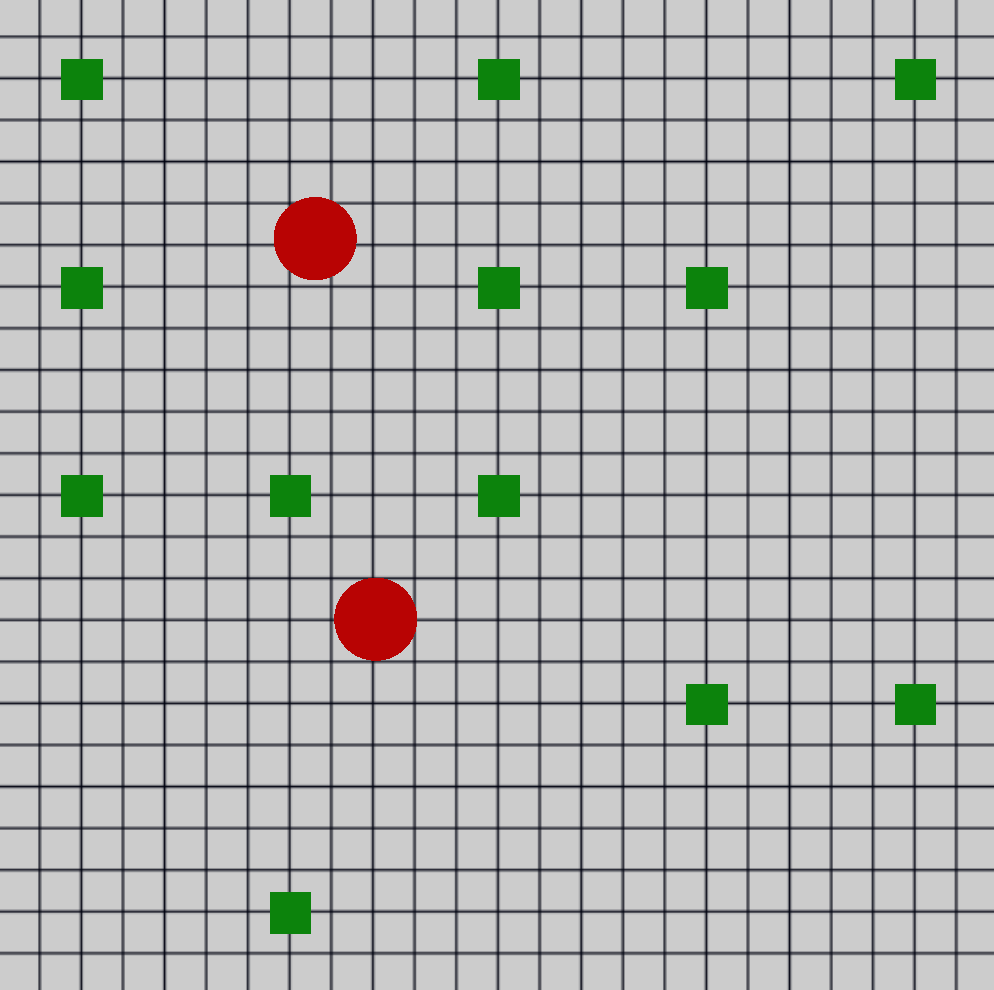
\includegraphics[width=0.49\textwidth,trim={1cm 9cm 1cm 5cm},clip]{figures/simple_picker_benchmark}
		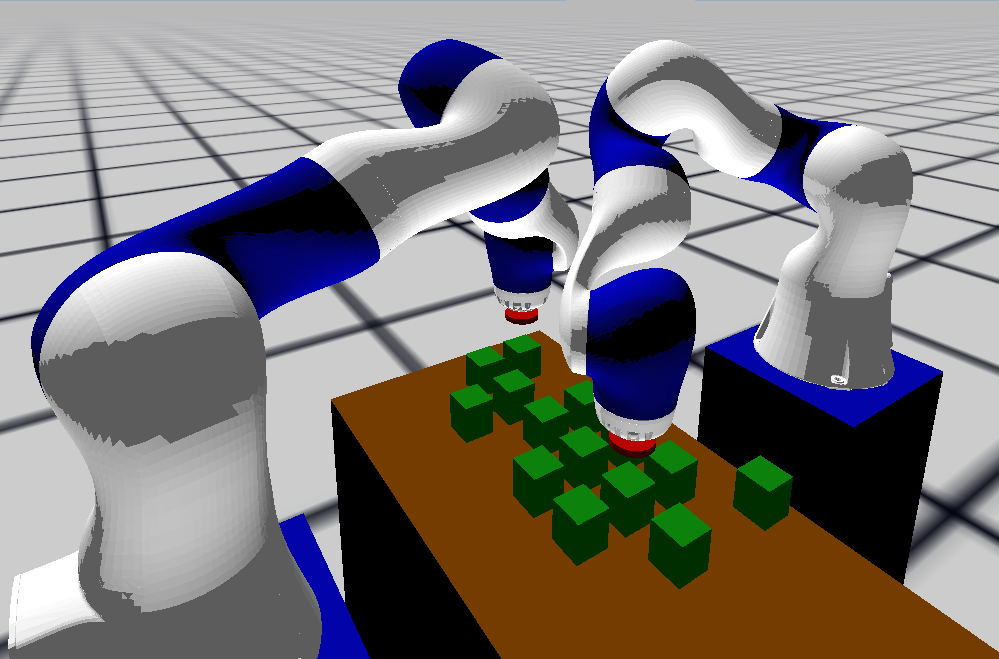
\includegraphics[width=0.47\textwidth]{figures/kuka_benchmark2}
%		\vspace{-.3in}
		\caption{\textit{Picker} and \textit{Manipulator} trials.}
		\label{fig:benchmarks}
%    \vspace{-.3in}
\end{figure*}
This section describes the experiments performed to evaluate the algorithms in two  domains shown in Fig \ref{fig:benchmarks}: a) simple picker and b) general manipulators.
%\begin{figure}[ht]
%	\centering
%	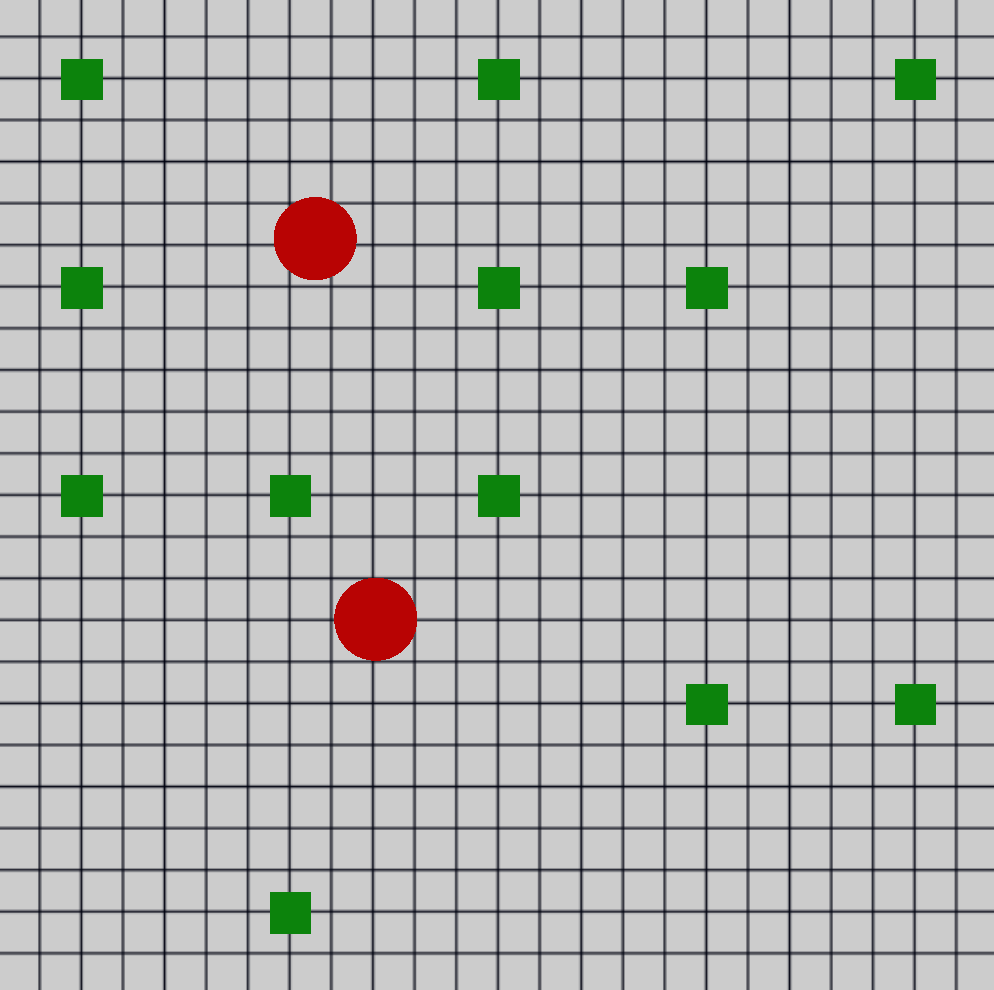
\includegraphics[width=1.9in]{figures/simple_picker_benchmark}
%	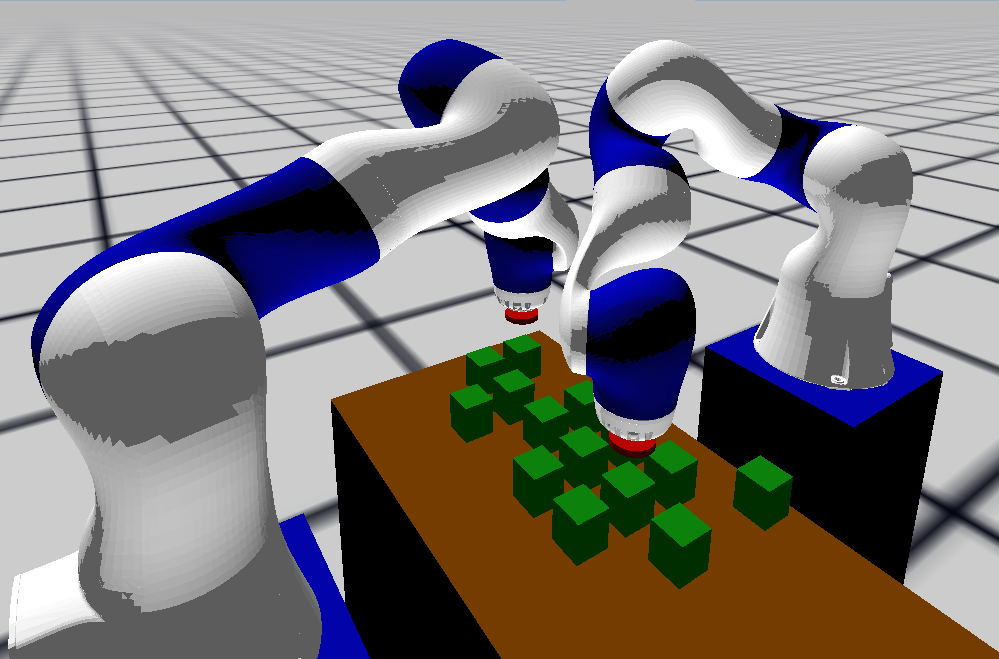
\includegraphics[width=1.8in]{figures/kuka_benchmark2}
%	\caption{The benchmarks: \textit{Simple Picker} and the \textit{General Manipulators} }
%	\label{fig:benchmarks}
%\end{figure}
In order to ensure monotonicity, the object starts and goals do not overlap. Uniform cuboidal objects simplify the grasping problem, though this is not a limitation of the methods. $ 50 $ random experiments were limited to $300s$ of computation time. The underlying $ \drrtstar $ motion planner is restricted to a max of $ 3s $ per plan.
A comparison point includes a random split method, which splits $ \objectset $ at random into two subsets and chooses an arbitrary ordering. Maximum of distances cost is compared to the single arm solution~\cite{193}. Computation times and success rates are reported. The trends in both experiments show that in the single-shot versions, exhaustive and \milp tend to time-out for larger $n$. Lazy variants scale much better for all the algorithms, and in some cases increase the success ratio due to retries. \algo has much better running time than exhaustive and \milp, and producing better and more solutions than random split. Overall, the results show a) our \milp succeeds more within the time limit than exhaustive, b) \algo scales the best among all the methods, and c) the cost of solutions from \algo is close to the optimal baseline, which is around half of the single arm cost.
% to demonstrate the gains from using multiple arms.  Overall, MILP scales better than exhaustive search, while finding optimal solutions. \algo scales better than the other methods, and finds high quality solutions. The lazy variants improve all the dual-arm methods.

%\subsection{Simple Picker}
%The results are shown in Figure~\ref{fig:disk}.
\textbf{Simple Picker}: This benchmark evaluates two disk robots hovering over a planar surface scattered with objects. The robots are only free to move around in a plane parallel to the resting plane of the objects, and the robots can pick up objects when they are directly above them. Fig~\ref{fig:disk}(\textit{top}) all runs up to $ 24 $ objects succeeded for \algo. \milp scales better than exhaustive. Lazy random split succeeds in all cases~(\textit{bottom}). In terms of solution costs~(\textit{middle}) exhaustive finds the true optimal. \milp matches exhaustive and \algo is competitive. In all experiments, \algo enjoys a success rate of 100\%.
% \kiril{What is the reason for low success rate of exhaustive and milp? Is it due to exceeding the time budget?} \kiril{This paragraph misses a statement that demonstrates the benefits of our approach: "In all experiments, \algo enjoys a success rate of \%100, while having much better running time than exhaustive and milp, and producing a higher cost solution than random split. Furthermore, \algo produces a plan whose cost is around half of the single arm plan cost." Similar statements should be added to the other experiments.}

%\subsection{General Manipulator}
%The results are shown in Figure~\ref{fig:kuka}.

\textbf{General Dexterous Manipulator}: The second benchmark sets up two \kuka arms across a table with objects on it. The objects are placed in the common reachable part of both arms' workspace, and only one top-down grasping configuration is allowed for each object pose. Here (Fig~\ref{fig:kuka}) a larger number of motion plans tend to fail, so the single shot variants show artifacts of the randomness of \drrtstar in their success rates. 
% The lazy iterative variants show the robust scalability. 
Random split performs the worst since it is unlikely to chance upon valid motion plans. Single shot exhaustive and \milp scale poorly because of expensive motion planning.
Interestingly, motion planning infeasibility reduces the size of the exhaustive search tree.
The solution costs \textit{(middle)} substantiate benefits of the use of two arms. The computation times \textit{(bottom)} again show the scalability of \algo, even compared to random split.
% In terms of cost. MILP scales to more objects but the computational overhead is more than \algo. Dual-arm solutions are significantly better than single arm.




\begin{figure*}[h!]
%\vspace{-0.2in}
	\centering
%	\includegraphics[width=2.1in]{figures/disk_solution}
%	\includegraphics[width=2.1in]{figures/disk_timing}
%	\includegraphics[width=2.1in]{figures/disk_more_solution}
%	\includegraphics[width=2.1in]{figures/disk_more_timing}

%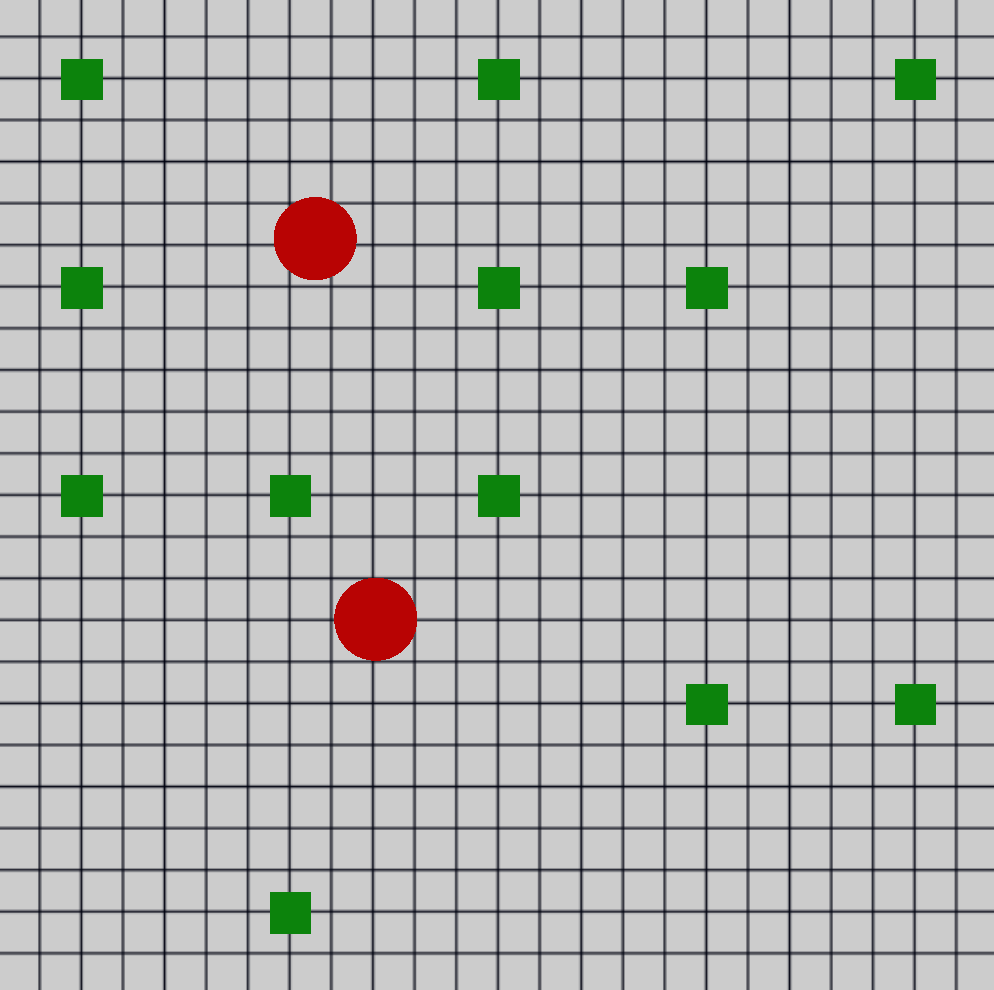
\includegraphics[width=0.48\textwidth,trim={1cm 9cm 1cm 5cm},clip]{figures/simple_picker_benchmark}\\
	
\includegraphics[width=0.6\textwidth]{figures/results/labels}
	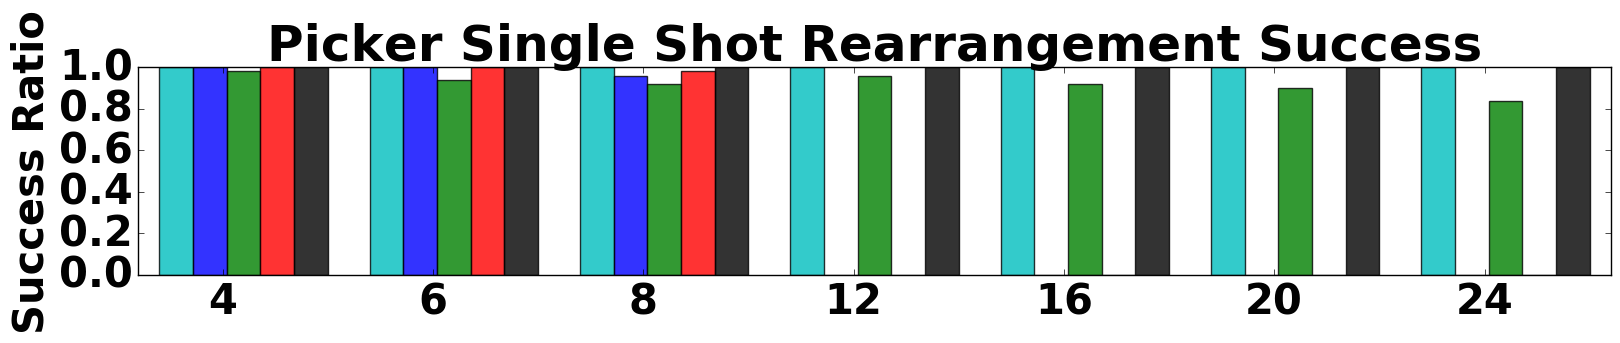
\includegraphics[width=0.48\textwidth]{figures/results/4_sp_ms_success}
	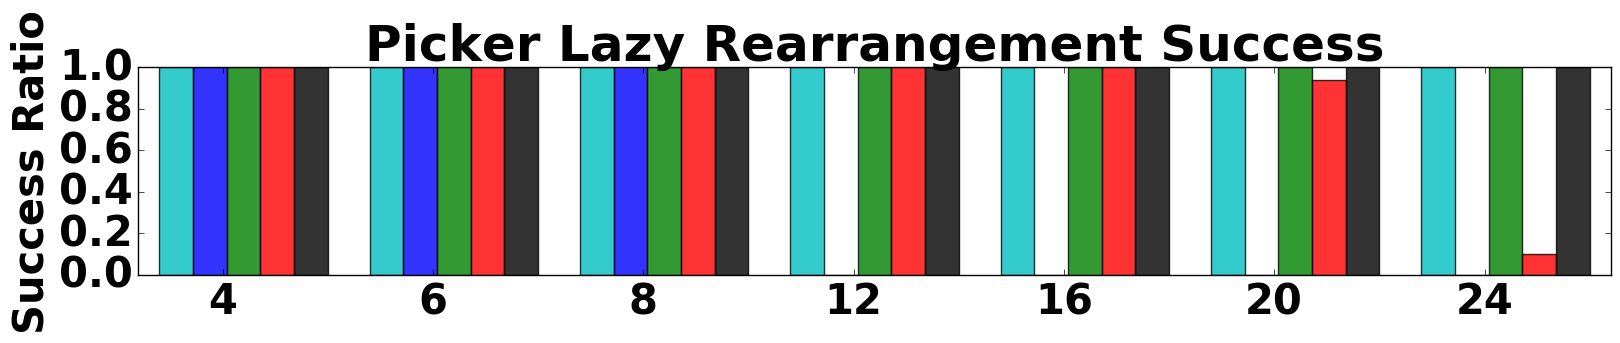
\includegraphics[width=0.48\textwidth]{figures/results/3_sp_lazy_ms_success}
	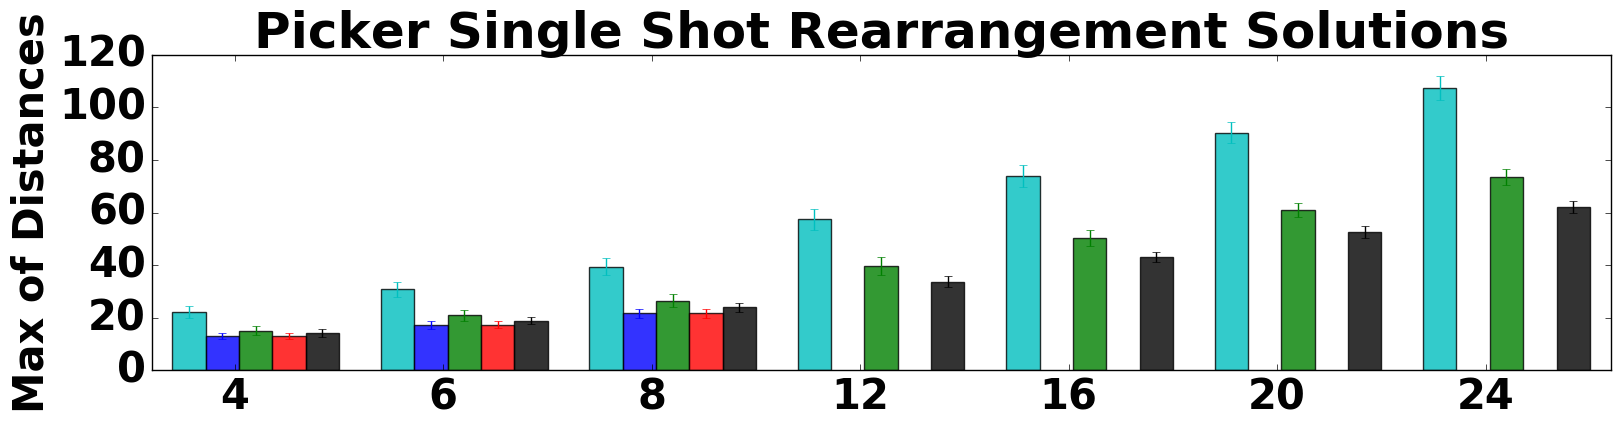
\includegraphics[width=0.48\textwidth]{figures/results/4_sp_ms_cost}
	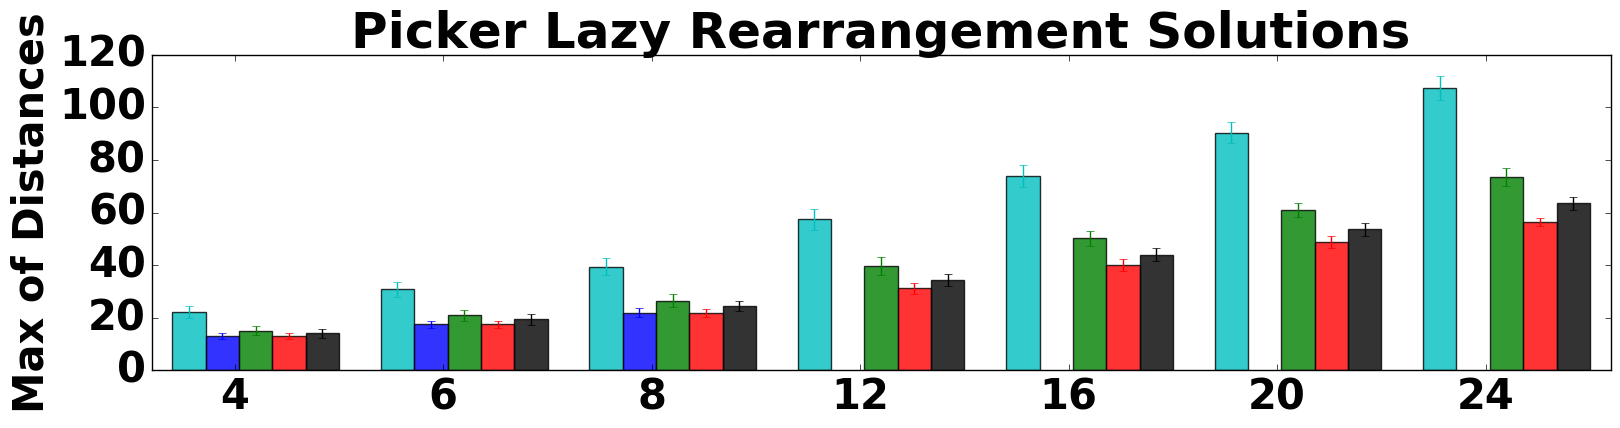
\includegraphics[width=0.48\textwidth]{figures/results/3_sp_lazy_ms_cost}
	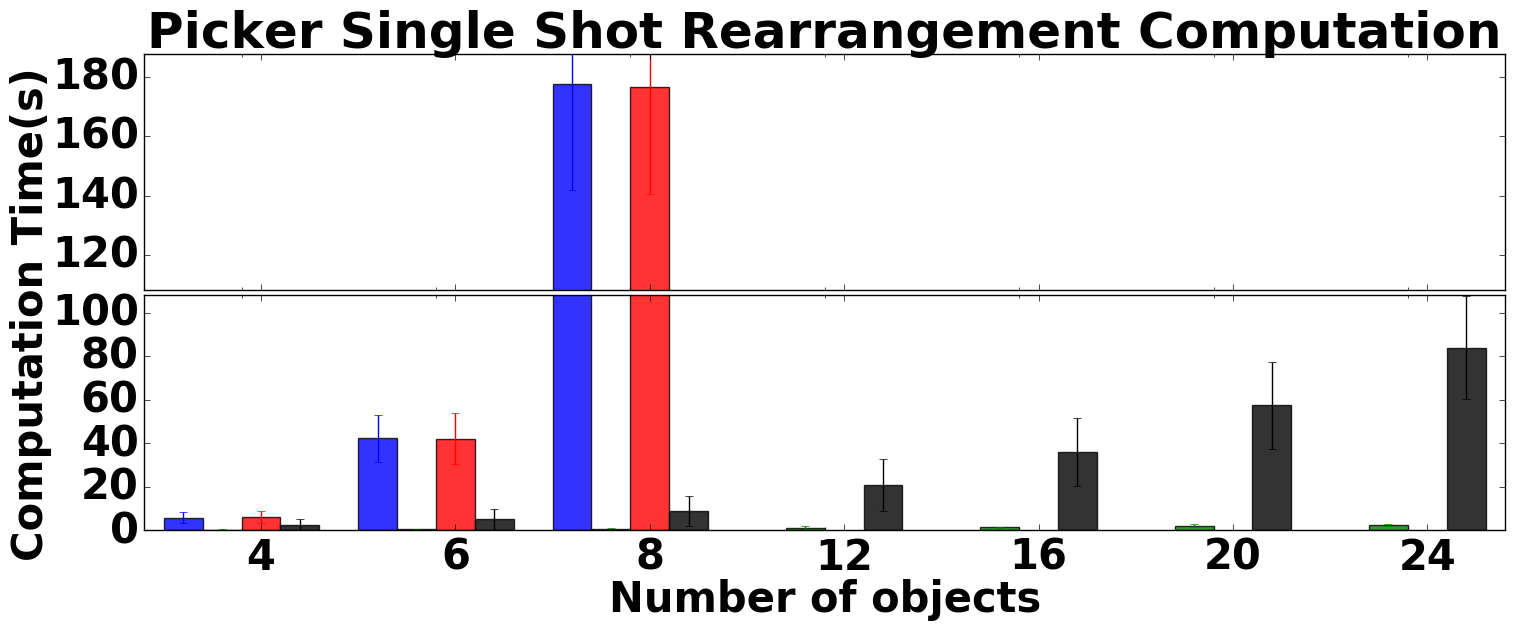
\includegraphics[width=0.48\textwidth]{figures/results/4_sp_ms_time}
	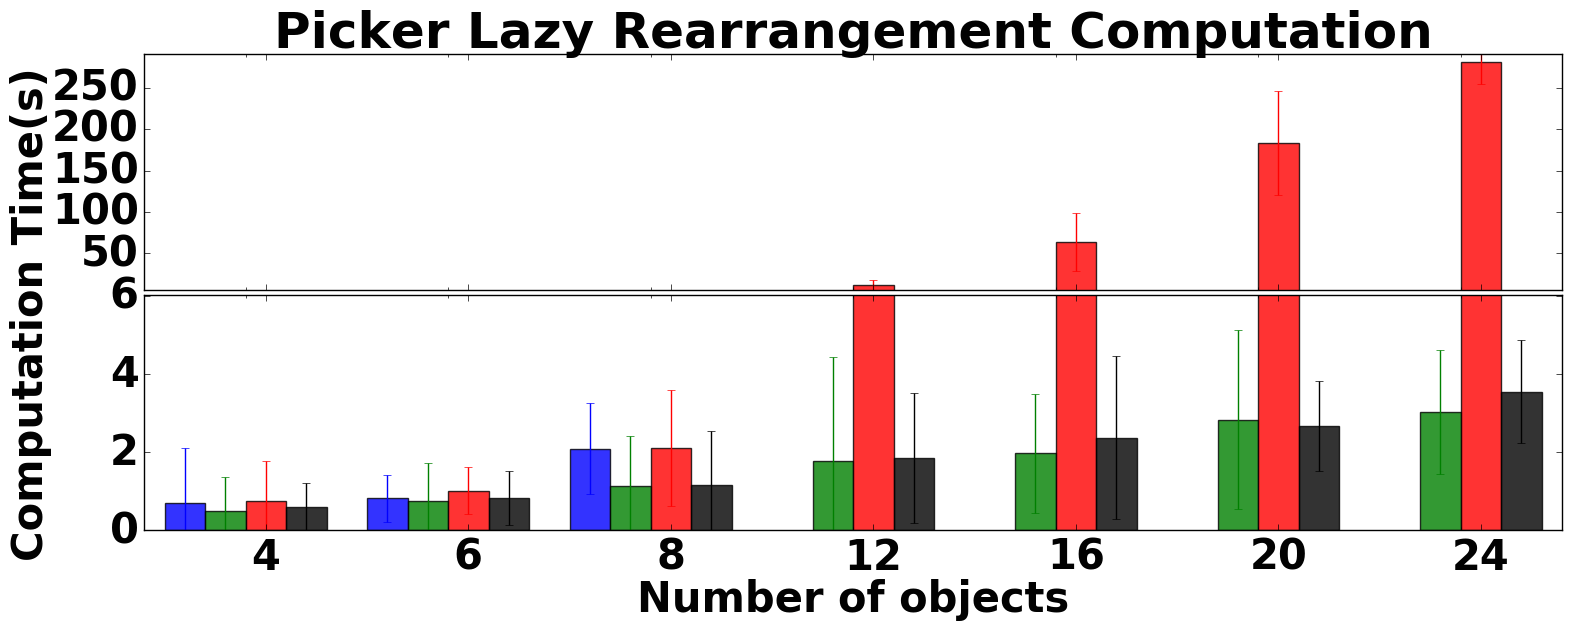
\includegraphics[width=0.48\textwidth]{figures/results/3_sp_lazy_ms_time}
%	\vspace{-0.15in}
	\caption{\textit{Simple Picker} results with success\textit{(top)}, solution costs\textit{(middle)}, and computation\textit{(bottom)} reported for single-shot\textit{(left)} and lazy\textit{(right)} versions of the methods}
%    \vspace{-0.3in}
	\label{fig:disk}
\end{figure*}

\begin{figure*}[h!]
%\vspace{-0.2in}
	\centering
%	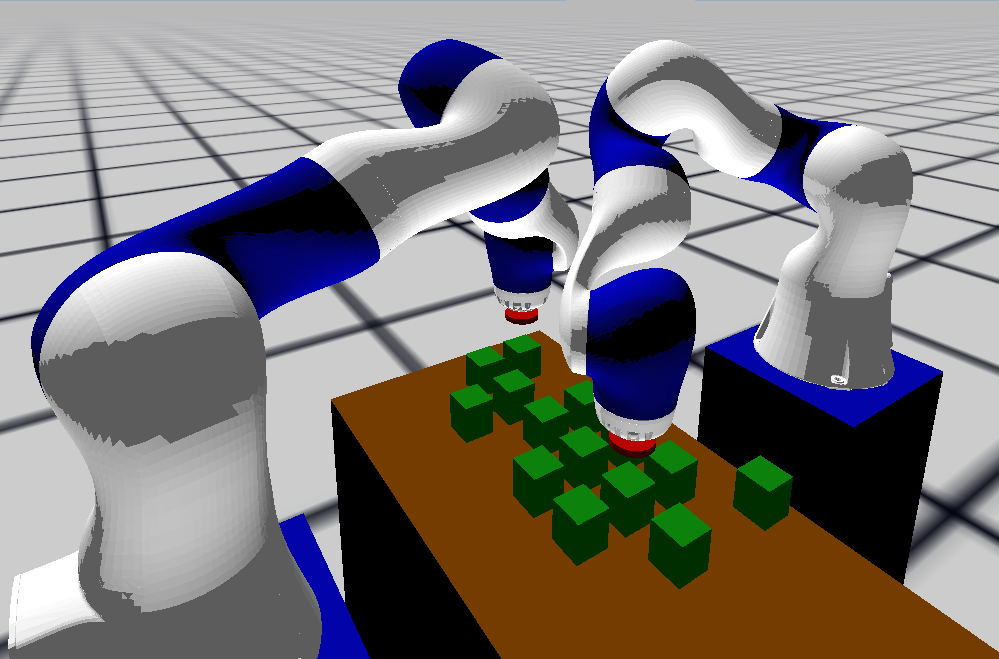
\includegraphics[width=0.48\textwidth]{figures/kuka_benchmark2}
	
\includegraphics[width=0.6\textwidth]{figures/results/labels}
	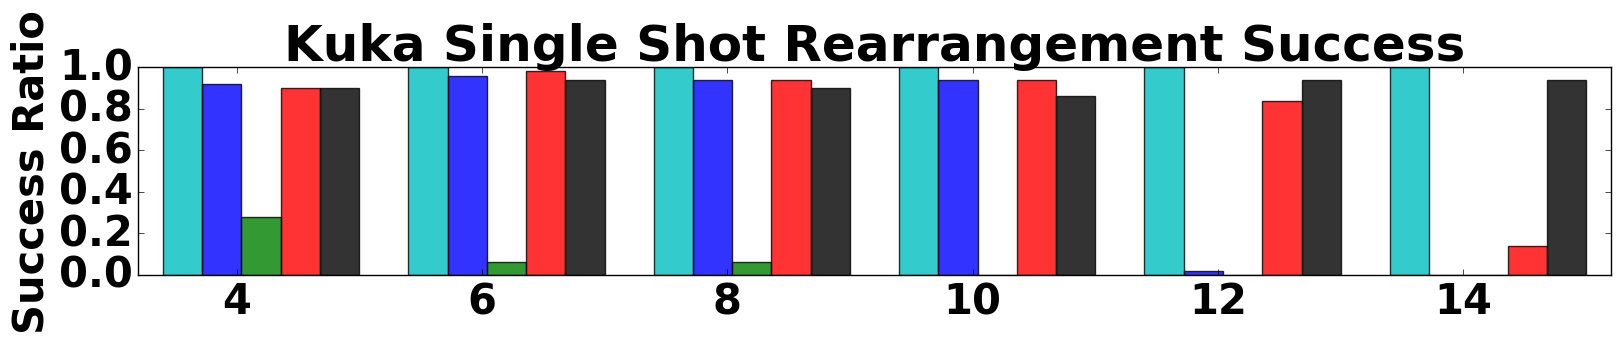
\includegraphics[width=0.48\textwidth]{figures/results/2_kuka_ms_success}
	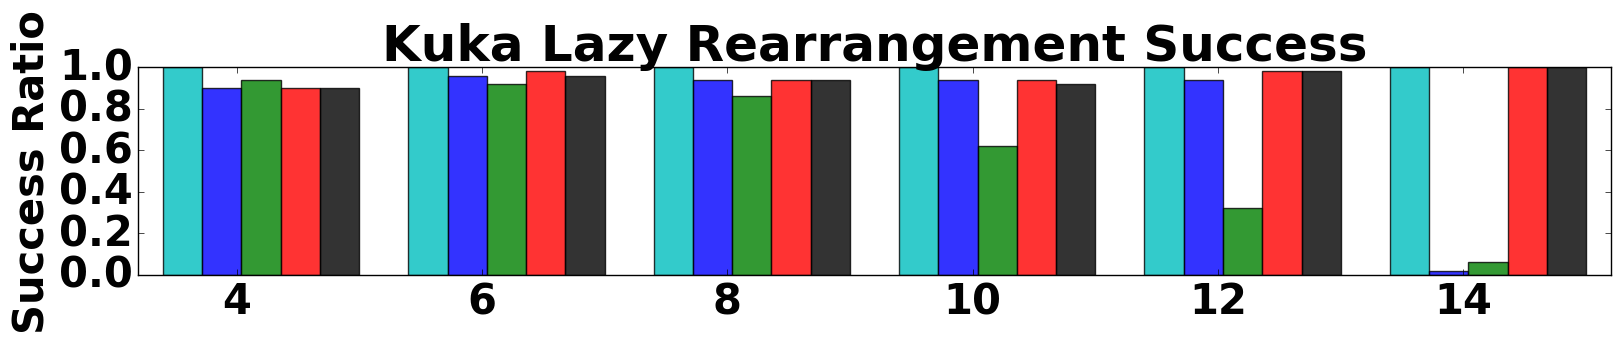
\includegraphics[width=0.48\textwidth]{figures/results/1_kuka_lazy_ms_success}
	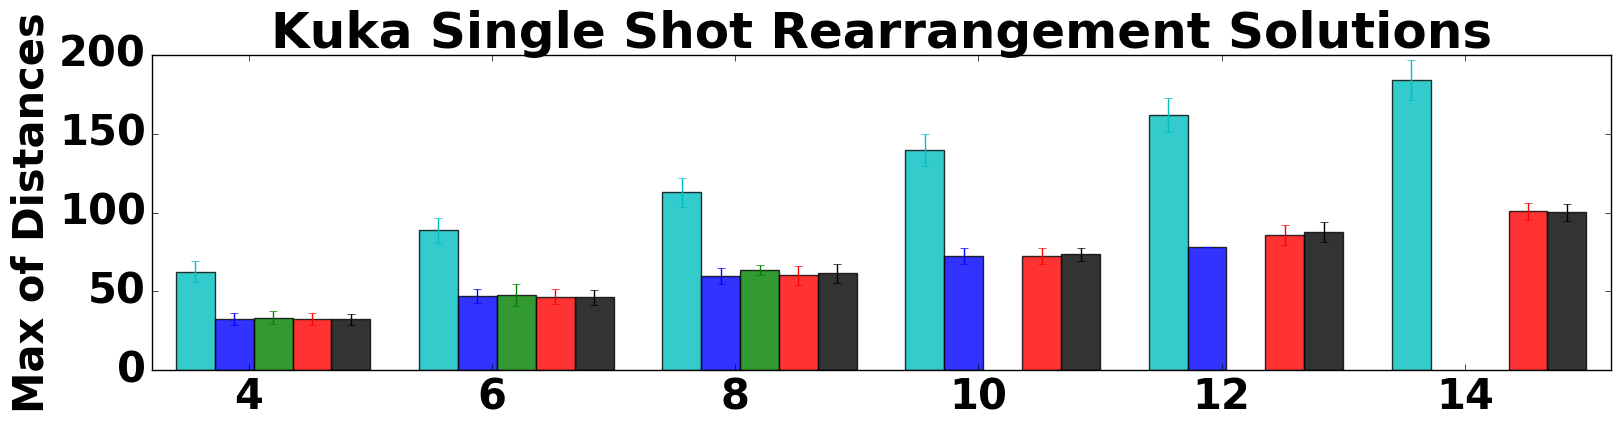
\includegraphics[width=0.48\textwidth]{figures/results/2_kuka_ms_cost}
	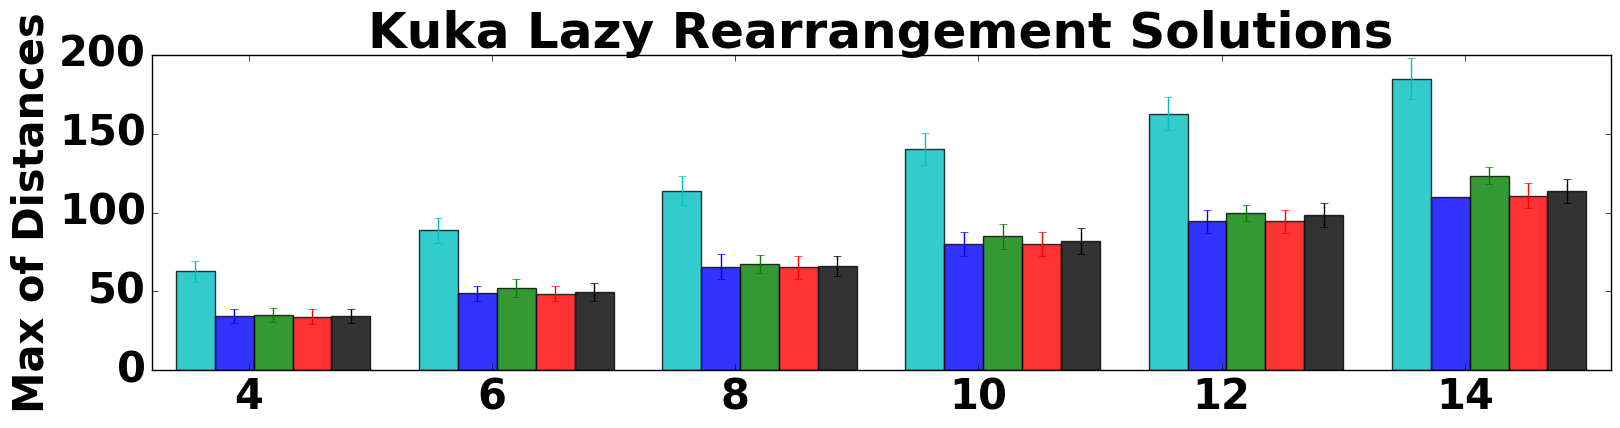
\includegraphics[width=0.48\textwidth]{figures/results/1_kuka_lazy_ms_cost}
	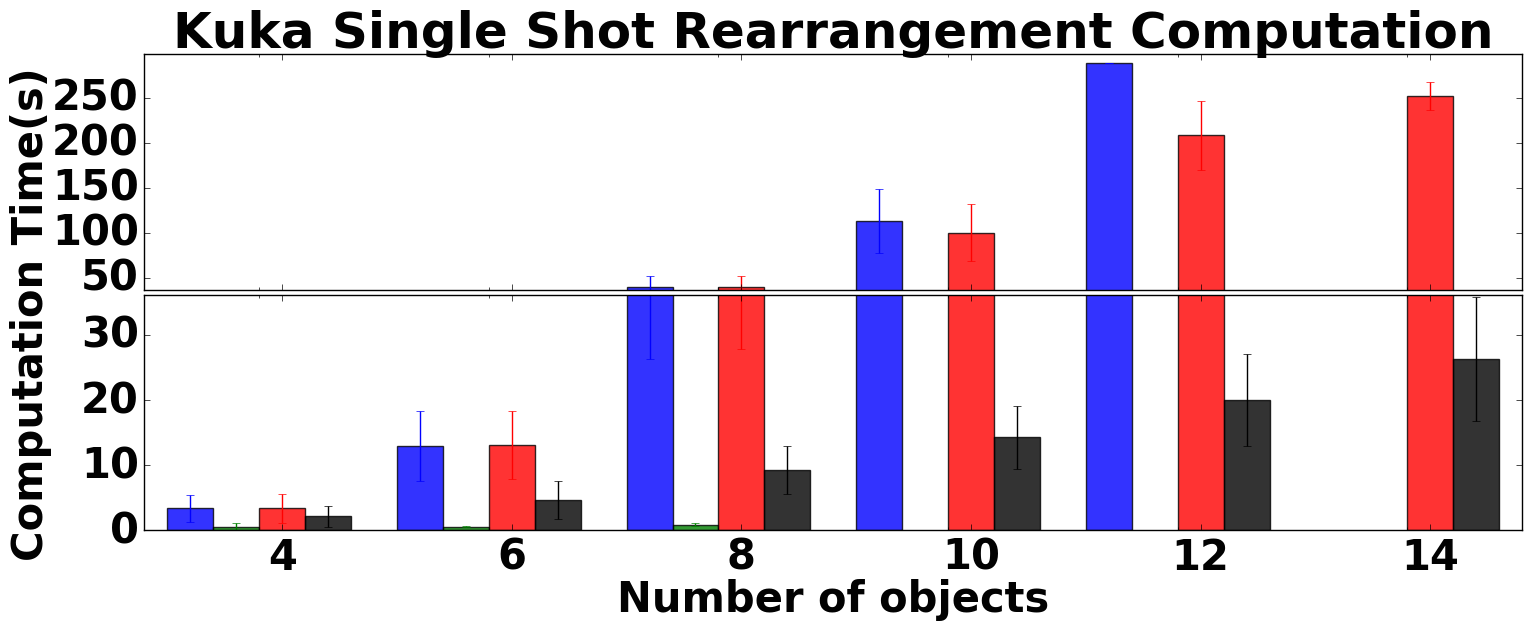
\includegraphics[width=0.48\textwidth]{figures/results/2_kuka_ms_time}
	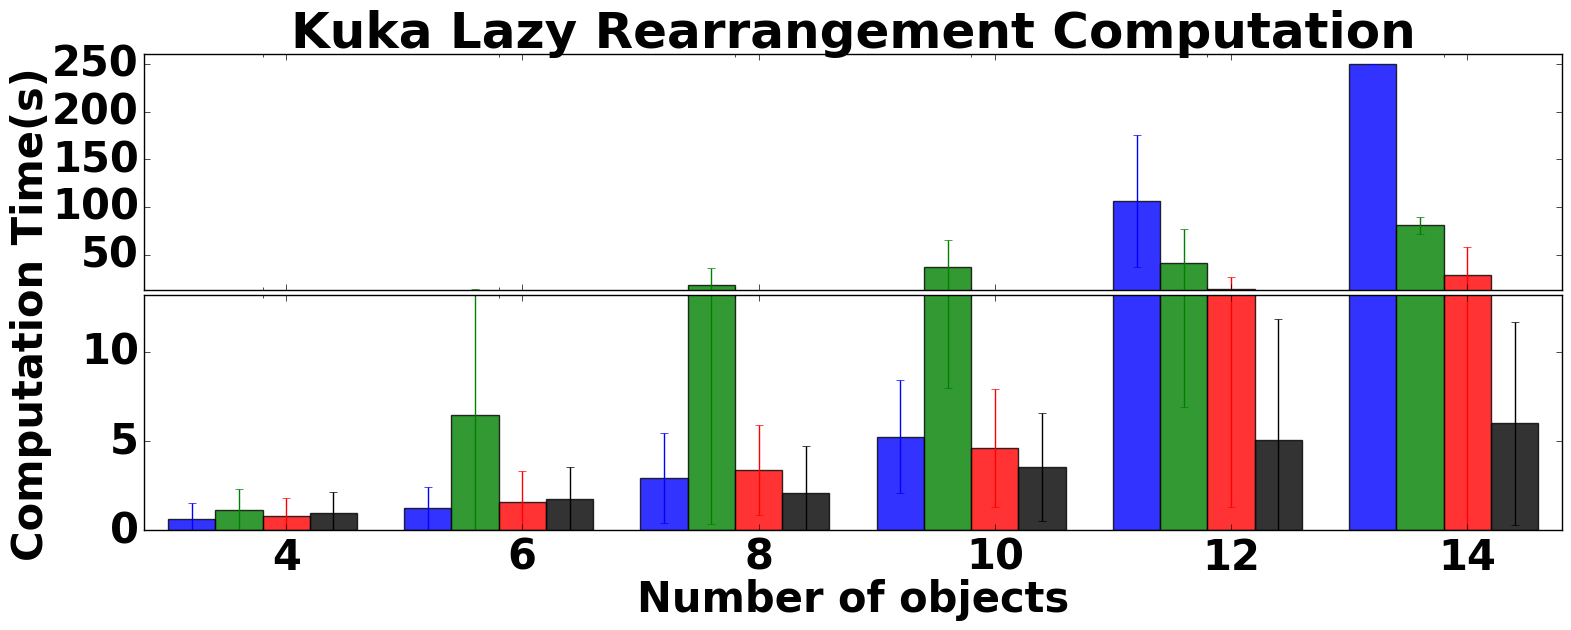
\includegraphics[width=0.48\textwidth]{figures/results/1_kuka_lazy_ms_time}
%	\vspace{-0.15in}
    \caption{\textit{\kuka}results with success\textit{(top)}, solution costs\textit{(middle)}, and computation\textit{(bottom)} reported for single-shot\textit{(left)} and lazy\textit{(right)} versions of the methods}
%    \vspace{-0.3in}
	\label{fig:kuka}
\end{figure*}

